\documentclass[b5paper,openany,multi={tikzpicture}]{standalone}
\usepackage{luatexja-preset}
\usepackage{tikz}
\usetikzlibrary{calc}
\usepackage{gachimuchimacro}
\begin{document}
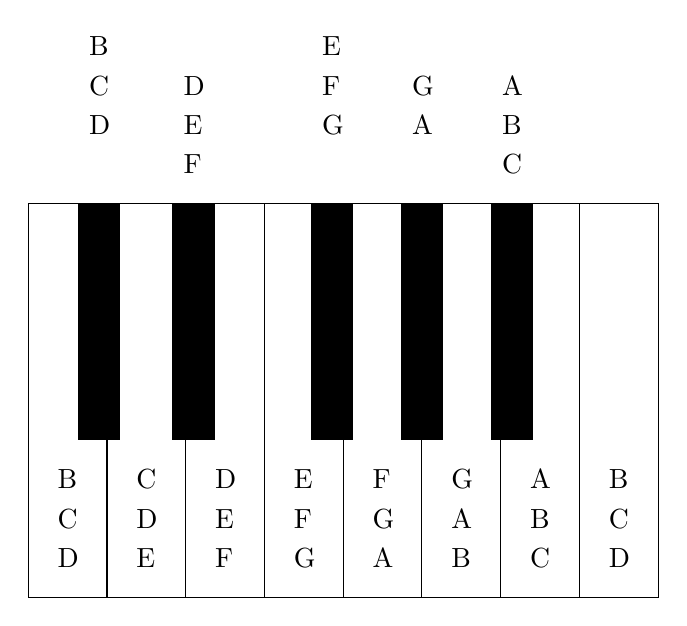
\begin{tikzpicture} % tikzpicture環境開始
\draw (0,0) rectangle (8,5);%オクターブ分の長方形
\foreach \num in{1,2,3,4,5,6,7}{\draw(\num,0) -- (\num,5);}%白鍵の区切り
\pgfmathdivide {9}{10}\coordinate (KURO1) at (\pgfmathresult,5);
\pgfmathdivide{21}{10}\coordinate (KURO2) at (\pgfmathresult,5);
\pgfmathdivide {27}{7}\coordinate (KURO3) at (\pgfmathresult,5);
\pgfmathdivide  {5}{1}\coordinate (KURO4) at (\pgfmathresult,5);
\pgfmathdivide {43}{7}\coordinate (KURO5) at (\pgfmathresult,5);
\fill ($(KURO1) + (-0.27, 0)$) rectangle +(0.54,-3);
\fill ($(KURO2) + (-0.27, 0)$) rectangle +(0.54,-3);
\fill ($(KURO3) + (-0.27, 0)$) rectangle +(0.54,-3);
\fill ($(KURO4) + (-0.27, 0)$) rectangle +(0.54,-3);
\fill ($(KURO5) + (-0.27, 0)$) rectangle +(0.54,-3);
\coordinate(C1) at (0.5 , 1);
\coordinate(D1) at (1.5 , 1);
\coordinate(E1) at (2.5 , 1);
\coordinate(F1) at (3.5 , 1);
\coordinate(G1) at (4.5 , 1);
\coordinate(A1) at (5.5 , 1);
\coordinate(H1) at (6.5 , 1);
\coordinate(C2) at (7.5 , 1);
\node at (C1) [right=-0.25cm] {C};
\node at (D1) [right=-0.25cm] {D};
\node at (E1) [right=-0.25cm] {E};
\node at (F1) [right=-0.25cm] {F};
\node at (G1) [right=-0.25cm] {G};
\node at (A1) [right=-0.25cm] {A};
\node at (H1) [right=-0.25cm] {B};
\node at (C2) [right=-0.25cm] {C};
%
\node(Des1) at ($(KURO1)+(0,1)$)   [right=-0.25cm] {D\aFlat};
\node(Es1)  at ($(KURO2)+(0,1)$)   [right=-0.25cm] {E\aFlat};
\node(Fes1) at ($(E1)   -(0,0.5)$) [right=-0.25cm] {F\aFlat};
\node(Ges1) at ($(KURO3)+(0,1)$)   [right=-0.25cm] {G\aFlat};
\node(As1)  at ($(KURO4)+(0,1)$)   [right=-0.25cm] {A\aFlat};
\node(B1)   at ($(KURO5)+(0,1)$)   [right=-0.25cm] {B\aFlat};
\node(Ces2) at ($(H1)   -(0,0.5)$) [right=-0.25cm] {C\aFlat};
%
\node(Deses1) at ($(C1)   -(0,0.5)$) [right=-0.25cm] {D\adFlat};
\node(Eses1)  at ($(D1)   -(0,0.5)$) [right=-0.25cm] {E\adFlat};
\node(Feses1) at ($(KURO2)+(0,0.5)$) [right=-0.25cm] {F\adFlat};
\node(Geses1) at ($(F1)   -(0,0.5)$) [right=-0.25cm] {G\adFlat};
\node(Ases1)  at ($(G1)   -(0,0.5)$) [right=-0.25cm] {A\adFlat};
\node(Bes1)   at ($(A1)   -(0,0.5)$) [right=-0.25cm] {B\adFlat};
\node(Ceses2) at ($(KURO5)+(0,0.5)$) [right=-0.25cm] {C\adFlat};
\node(Deses2) at ($(C2)   -(0,0.5)$) [right=-0.25cm] {D\adFlat};
%
\node(His0) at ($(C1)   +(0,0.5)$) [right=-0.25cm] {B\aSharp};
\node(Cis1) at ($(KURO1)+(0,1.5)$) [right=-0.25cm] {C\aSharp};
\node(Dis1) at ($(KURO2)+(0,1.5)$) [right=-0.25cm] {D\aSharp};
\node(Eis1) at ($(F1)   +(0,0.5)$) [right=-0.25cm] {E\aSharp};
\node(Fis1) at ($(KURO3)+(0,1.5)$) [right=-0.25cm] {F\aSharp};
\node(Gis1) at ($(KURO4)+(0,1.5)$) [right=-0.25cm] {G\aSharp};
\node(Ais1) at ($(KURO5)+(0,1.5)$) [right=-0.25cm] {A\aSharp};
\node(His1) at ($(C2)   +(0,0.5)$) [right=-0.25cm] {B\aSharp};
%
\node(Hisis0) at ($(KURO1)+(0,2.0)$) [right=-0.25cm] {B\adSharp};
\node(Cisis1) at ($(D1)   +(0,0.5)$) [right=-0.25cm] {C\adSharp};
\node(Disis1) at ($(E1)   +(0,0.5)$) [right=-0.25cm] {D\adSharp};
\node(Eisis1) at ($(KURO3)+(0,2.0)$) [right=-0.25cm] {E\adSharp};
\node(Fisis1) at ($(G1)   +(0,0.5)$) [right=-0.25cm] {F\adSharp};
\node(Gisis1) at ($(A1)   +(0,0.5)$) [right=-0.25cm] {G\adSharp};
\node(Aisis1) at ($(H1)   +(0,0.5)$) [right=-0.25cm] {A\adSharp};
\end{tikzpicture} % tikzpicture環境終了
\end{document}
